\begin{figure}[ht]
	\centering
	\footnotesize

	\psfrag{x}[l][l] {$x$}

	\psfrag{x1}[l][l] {$x_{j}$}
	\psfrag{x2}[l][l] {$x_{j-1}$}
	\psfrag{x3}[l][l] {$x_{j-2}$}
	\psfrag{x4}[l][l] {$x_{j-3}$}
	\psfrag{x5}[l][l] {$x_{j-4}$}
	\psfrag{x6}[l][l] {$x_{j-5}$}

	% \psfrag{r}[l][l] {$\rho(x,t)$}
	% \psfrag{r1}[l][l] {$\rho(x_{1},t)$}
	% \psfrag{r2}[l][l] {$\rho(x_{2},t)$}

	\psfrag{t0}[l][l] {$t=0$}
	\psfrag{tla}[l][l] {$t>0$}

	\psfrag{t}[l][l] {$t$}
	\psfrag{t1}[l][l] {$t_{n+1}$}
	\psfrag{t2}[l][l] {$t_{n}$}

	\psfrag{A}[l][l] {$A$}
	\psfrag{B}[l][l] {$B$}
	\psfrag{C}[l][l] {$C$}
	\psfrag{D}[l][l] {$D$}
	\psfrag{E}[l][l] {$E$}

	\psfrag{pA}[l][l] {$A(x_j,t_n)\,\checkmark$}
	\psfrag{pB}[l][l] {$B(x_{j-1},t_{n-1})\,\checkmark$}
	\psfrag{pC}[l][l] {$C(x_{j},t_{n-1})\,\checkmark$}
	\psfrag{pD}[l][l] {$D(x_D,t_D)\,?$}
	\psfrag{pE}[l][l] {$E(x_E,t_E)\, ?$}

	\psfrag{l1}[l][l] {$l_1$}
	\psfrag{l2}[l][l] {$l_2$}

	\psfrag{a1}[l][l] {$a>0$}
	\psfrag{a2}[l][l] {$a<0$}

	\psfrag{c1}[c][c] {$\text{Case }1:\ u_{L} > u_{R} > 0$}
	\psfrag{c21}[c][c] {$\text{Case }2.1:\ (u_{L} > 0 > u_{R}) \wedge  \left|u_{L}\right| > \left|u_{R}\right|$}
	\psfrag{c22}[c][c] {$\text{Case }2.2:\ (u_{L} > 0 > u_{R}) \wedge  \left|u_{L}\right| < \left|u_{R}\right|$}
	\psfrag{c3}[c][c] {$\text{Case }3:\ 0 > u_{L} > u_{R}$}

	\psfrag{uL}[c][c] {$u_{L}$}
	\psfrag{uR}[c][c] {$u_{R}$}

	\psfrag{L}[c][c] {$C_L$}
	\psfrag{R}[c][c] {$C_R$}

	\psfrag{ucaL}[c][c] {$\displaystyle (C_L):\ t=\frac{1}{u_{L}}x-\frac{x_{0}}{u_{L}}$}
	\psfrag{ucaR}[c][c] {$\displaystyle (C_R):\ t=\frac{1}{u_{R}}x-\frac{x_{0}}{u_{R}}$}

	\psfrag{p1}[l][l] {$x_{j}$}
	\psfrag{p2}[l][l] {$x_{j+1}$}

	\psfrag{ur1}[l][l] {$u_{j}$}
	\psfrag{ur2}[l][l] {$u_{j+1}$}

	\psfrag{ul1}[l][l] {$u_{j-1}$}
	\psfrag{ul2}[l][l] {$u_{j}$}

	\psfrag{dx3}[l][l] {$\dots$}
	\psfrag{dt3}[l][l] {$\vdots$}

	\psfrag{s}[c][c] {$s^{RH}$}

	\psfrag{mt}[l][l] {$\displaystyle u_{j}^{n+1} = u_{j}^{n} + \frac{a\Delta t}{\Delta x}\left(u_{j-1}^{n}-u_{j}^{n}\right)$}

	\psfrag{eq}[l][l] {$\displaystyle u_{t} + au_{x} = 0 \quad (a>0)$}

	% \psfrag{to}[l][l] {$t = 0$}
	% \psfrag{ti}[l][l] {$t \rightarrow +\infty$}

	% \psfrag{i1}[c][c] {$\displaystyle I_{1} = \int_{0}^{+\infty}\int_{-\infty}^{+\infty} \left(\cdot\right)dxdt$}
	% \psfrag{i2}[c][c] {$\displaystyle I_{2} = \int_{-\infty}^{+\infty}\int_{0}^{+\infty} \left(\cdot\right)dtdx$}

	% \psfrag{i1}[c][c] {$\displaystyle I_{1} = \int_{0}^{\mathscr{T}}\int_{\mathscr{D}} \left(\cdot\right)dxdt$}
	% \psfrag{i2}[c][c] {$\displaystyle I_{2} = \int_{\mathscr{D}}\int_{0}^{\mathscr{T}} \left(\cdot\right)dtdx$}

	% \psfrag{x}[l][l] {$x$}
	% \psfrag{xl}[r][r] {$x\rightarrow -\infty$}
	% \psfrag{xr}[l][l] {$x\rightarrow +\infty$}

	\psfrag{oh}[l][l] {$O$}
	% \psfrag{id}[l][l] {$\text{Integration direction}$}

	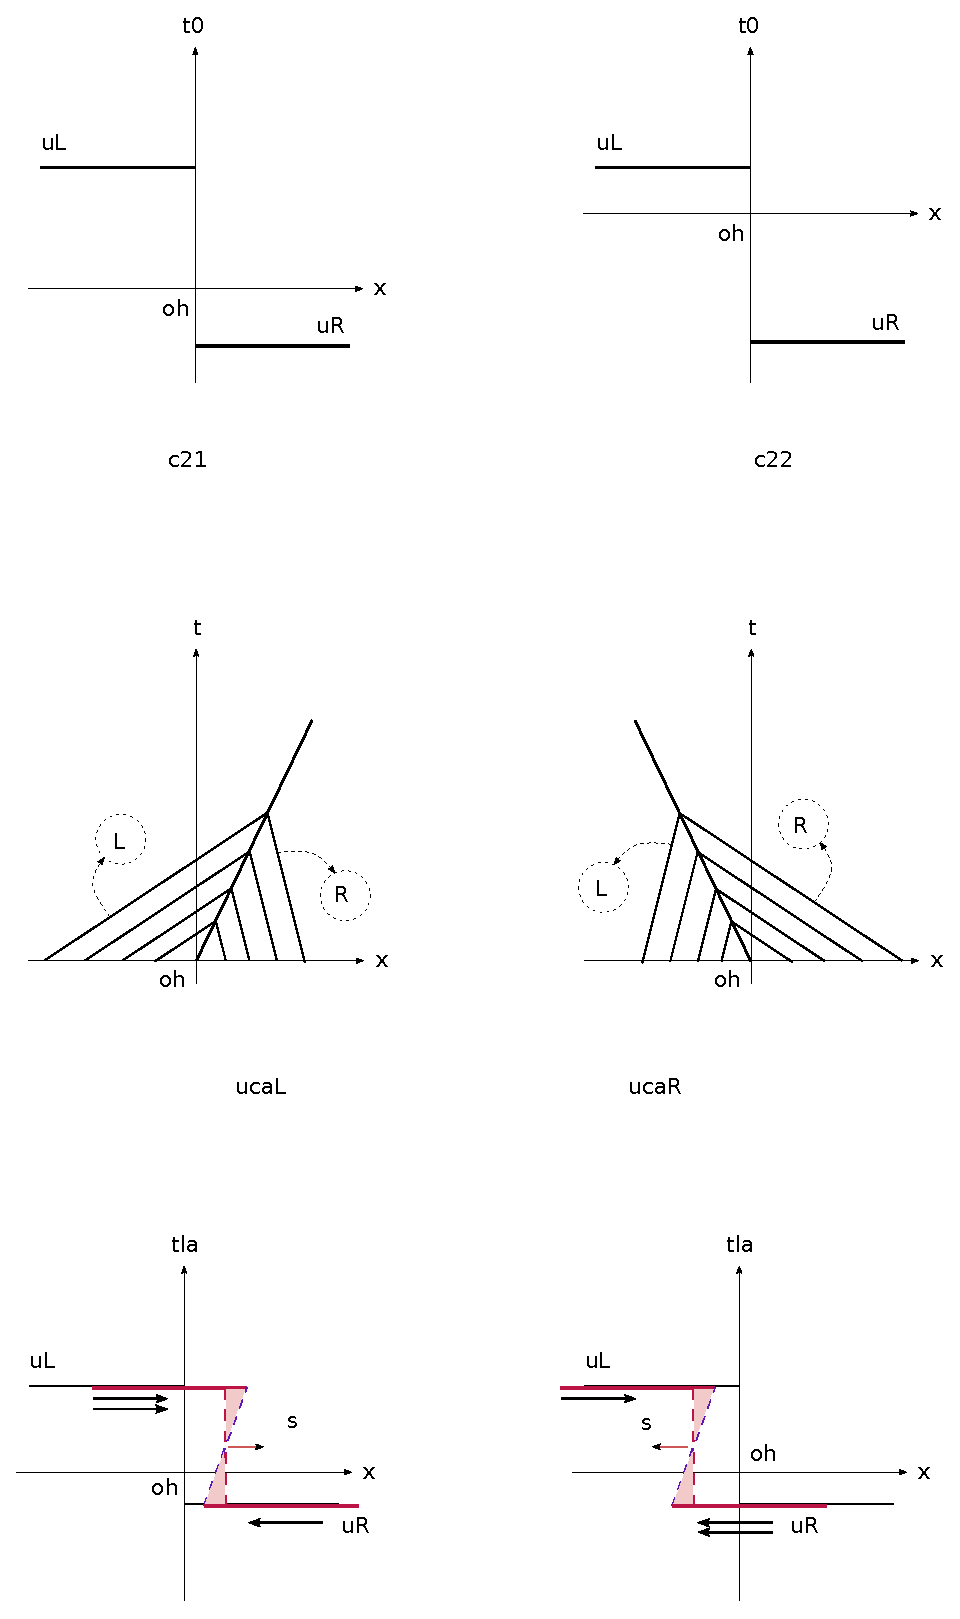
\includegraphics[width=0.7\textwidth]{RiemannAllCasesLR_set2.eps}
	\caption{Riemann problem with $u_{L} >u_{R}$:  IC, Characteristics, Solution.}
	\label{\LABEL}
\end{figure}